\documentclass[a4paper,10pt]{report}
\usepackage[utf8]{inputenc}
\usepackage{amssymb}
\usepackage{amsthm}
\usepackage{amsmath}
\usepackage{graphicx}
\usepackage{subcaption}
\usepackage{subfig}


\setlength{\parindent}{0pt}

\begin{document}
\title{Lab 5: RC Circuits}
\author{Adam Olson, Nick Lonsdale, Zack Garza}
\maketitle
\tableofcontents

\begin{abstract}
	This is some abstract stuff.
\end{abstract}

\chapter{Introduction}
This is an introduction.

\chapter{Theory}

\chapter{Equipment List}
	\begin{enumerate}
		\item Function Generator
		\item Digital Oscilloscope (2 Channel)
		\item Breadboard
		\item Resistors;
			\begin{enumerate}
				\item 1x 1.0 k$\Omega$, ($\frac{1}{4}$W)
				\item 2x 10.0 k$\Omega$, ($\frac{1}{4}$W)
			\end{enumerate}
		\item Capacitors
			\begin{enumerate}
				\item 1x .01 $\mu$F
				\item 1x 100 pF
				\item 2x .001 $\mu$F
			\end{enumerate}
	\end{enumerate}

\chapter{Methodology}
	\section{Differentiator}
	\section{Integrator}
	\section{Low-Pass Filter}
	\section{High-Pass Filter}
	\section{Band-Pass Filter}

\chapter{Results}
	\section{Differentiator}
	\section{Integrator}
	\section{Low-Pass Filter}
	\section{High-Pass Filter}
	\section{Band-Pass Filter}


\chapter{Appendicies}
	\section{Derivations}
	\section{Equipment Photographs}
	\section{Circuit Diagrams}
	\noindent\begin{figure}
		\null\hfill
		\begin{subfigure}{.5\linewidth}
			\centering
			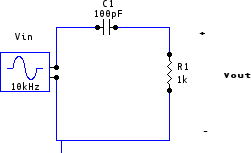
\includegraphics[width=.9\linewidth]{./Circuits/Differentiator.png}
			\caption{}
			\label{fig:sub1}
		\end{subfigure}%
		\hfill
		\begin{subfigure}{.5\linewidth}
			\centering
			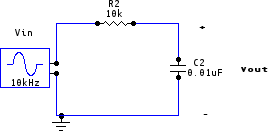
\includegraphics[width=.9\linewidth]{./Circuits/Integrator.png}
			\caption{}
			\label{fig:sub2}
		\end{subfigure}\hfill\null\\[1ex]\null\hfill
		\begin{subfigure}{.5\linewidth}
			\centering
			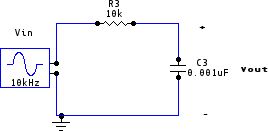
\includegraphics[width=.9\linewidth]{./Circuits/LowPassFilter.png}
			\caption{}
			\label{fig:sub3}
		\end{subfigure}\hfill
		\begin{subfigure}{.5\linewidth}
			\centering
			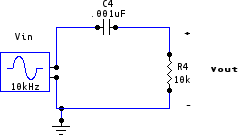
\includegraphics[width=.9\linewidth]{./Circuits/HighPassFilter.png}
			\caption{}
			\label{fig:sub3}
		\end{subfigure}\hfill\null\\[1ex]\null\hfill
		\begin{subfigure}{\linewidth}
			\centering
			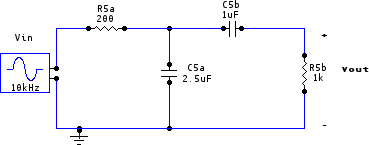
\includegraphics[width=.9\linewidth]{./Circuits/BandPassFilter.png}
			\label{fig:BandPassFilter}
			\caption{Band Pass Filter}
		\end{subfigure}\hfill\null
		\caption{Circuit Diagrams}
		\label{fig:test}

	\end{figure}

	\section{Circuit Photographs}

\end{document}